\documentclass[report,11pt]{elsarticle}
%\documentclass{article}[11pt,a4]
%\documentclass[11pt]{article}

\usepackage[lined,linesnumbered]{algorithm2e}
\usepackage{a4wide}
\usepackage{ae}
\usepackage[czech,english]{babel}
\usepackage[utf8x]{inputenc}
\usepackage[T1]{fontenc}
\usepackage{graphicx}
\usepackage{url}
\usepackage{pdfpages}

\usepackage{listings}

\paperwidth=210 true mm
\paperheight=297 true mm
\pdfpagewidth=210 true mm
\pdfpageheight=297 true mm

% Pro cestinu zakomentuj nasledujici radek
%\selectlanguage{english}
% Pro anglictinu zakomentuj nasledujici radek
\selectlanguage{czech}

% Znakem procenta zacina komentovan

%%%% Pokud chcete
%%% odkomentu
%\usepackage[lined,linesnumbered]{algorithm2e}
%\usepackage{algorithm2e}
% Tento b
%\usepackage{ctable}
%\DeclareGraphicsExtensions{.pdf}

% \renewcommand{\figurename}{Obrázek}
\addto\captionsenglish{%
  \renewcommand{\figurename}{Obrázek}
  \renewcommand{\lstlistingname}{Fragment kódu}
  \renewcommand{\partname}{Část}
}

\begin{document}

\begin{frontmatter}

\title{Diplomová práce\\ Jazyk pro definici uživatelského rozhraní}

\author{Michal Hotovec\footnote{A4M39SVP -- Michal Hotovec, zimní semestr 2014/15}\\
Katedra pořítačové grafiky a interakce,\\ Fakulta elektrotechnická, ČVUT Praha
}

\date{}



\end{frontmatter}

%\maketitle

%% \input{./section1.tex}
%% \input{./section2.tex}
%% \input{./section3.tex}
%% \input{./section4.tex}
%% \input{./section5.tex}

%%%% -------------------------------------------------------- 
\section{\label{SEC:Intro}Zadání}
Úkolem řešitele je studium nástrojů pro tvorbu moderních grafických uživatelských rozhraní.
Student se zvlášť zaměří na jazyk QML. Výsledkem práce je jazyk co nejvíce podobný QML,
nicméně přímo integrovatelný do C/C++ aplikací. Navrhnutý jazyk student popíše gramatikou a
implementuje jeho překladač do pomocného C/C++ kódu. Výsledky své práce student předvede na
C/C++ aplikaci obsahující jím vytvořené statické uživatelské rozhraní.\\
Pokyny pro vypracování:
\begin{enumerate}
\item Důkladně nastudujte jazyk QML.
\item Popište vlastnosti jazyka QML, shrňte jeho klady a zápory.
\item Z QML odvoďte jazyk vhodný k přímé integraci do C/C++ aplikací.
\item Vzniklý jazyk popište gramatikou.
\item Implementujte překladač vzniklého jazyka, který ze vstupních zdrojových souborů vytvoří
validní C/C++ zdrojový kód.
\item Funkčnost demonstrujte na jednoduché grafické aplikaci obsahující takto vytvořené statické
uživatelské rozhraní.
\end{enumerate}

\section{\label{SEC:Intro}Úvod}
%\section{\label{SEC:Intro}Introduction}
Cílem této práce bylo vytvořit jazyk pro tvorbu grafického uživatelského rozhraní (GUI), který by poskytoval funkčnost podobnou jazyku QML. Ale oproti jazyku QML, který je interpretovaný, půjde vytvořený jazyk přeložit do zkompilovatelného kódu C/C++, čímž výsledná aplikace dosáhne vyšší rychlosti. Součástí práce také bylo vytvořit překladač pro daný jazyk, který ověří validitu vstupu a přeloží jej do kódu C/C++, který půjde integrovat do  C/C++ aplikace a spustit. Tato aplikace by následně měla zobrazit jednoduché GUI.



\part{\label{CH:aa}Rešerše}

\section{\label{SEC:QML}Jazyk QML}
\subsection{Qt}
Qt je multi-platformní open-source knihovna sloužící k vývoji především GUI aplikací v jazyce C++. Aplikace se vyznačují tzv. nativním vzhledem GUI, což znamená, že se pro grafické rozhraní využívají standardní nástroje/knihovny poskytované operačním systémem. Tímto je dosaženo obdobného vzhledu, jaký mají standardní aplikace pro daný operační systém. Jednou z výhod této knihovny je, že je svou rychlostí takřka srovnatelná s nativními knihovnami pro GUI, použije-li se imperativně definované GUI. Součástí Qt je Qt Quick, což je soubor technologií sloužících k tvorbě deklarativního GUI.\\
Qt poskytuje vývojové prostředí Qt creator, které lze použít pro vývoj C++ aplikací využívající prvky Qt nebo aplikací Qt Quick. Součástí Qt creator je vizuální debuger C++, editor kódu, grafický editor pro uživatelské rozhraní, interpret pro jazyk QML a debugger pro jazyk QML.

\subsection{Qt Quick}
Qt Quick je soubor technologií sloužících k tvorbě deklarativního GUI. Poskytuje sadu GUI elementů, deklarativní jazyk QML a modul Qt declarative. Qt declarative slouží jako modul pro využití QML v C/C++ aplikacích, který za běhu rozparsuje vstup ve formátu QML a sestaví podle něj GUI s využitím funkčnosti poskytovanou Qt. Jeho součástí je interpret jazyka JavaScript, který umožňuje evaluaci JavaScript kódu ve funkcích definovaných v QML souboru. Qt declarative GUI od aplikační logiky C++. K datům vytvořených v QML lze přistupovat, v C++ části aplikace a naopak prostřednictvím tohoto modulu.

\subsection{QML}
QML je jazyk vycházející z jazyka JavaScript. Jedná se o jazyk pro deklaraci hierarchického GUI, na vrcholu hierarchie je vždy jediný element a všechny ostatní elementy jsou na něj navázány ve stromové struktuře. Každý element může mít teoreticky neomezené množství potomků (elementy, jež se nacházejí v hierarchii přímo pod ním), avšak může mít nanejvýš jednoho rodiče (element, který se nachází v hierarchii přímo nad ním). Pouze kořenový element na vrcholu hierarchie nemá žádného rodiče.


\subsubsection{Syntaxe}
Základní syntaxe je ilustrována viz. Fragment kódu \ref{lst:qml1}.
\begin{lstlisting}[frame=single,caption=Tvorba dvou jednoduchých elementů pomocí jazyka QML.,label=Tvorba dvou jednoduchých elementů pomocí jazyka QML.,label=lst:qml1]
Rectangle
{
	width : 100; height : 100
	Image
	{
		source : "img.jpg"
	}
}
\end{lstlisting}
Soubor s tímto kódem vytvoří dva GUI elementy. Kořenovým prvkem je element typu Rectangle, jehož potomkem je element typu Image. Element typu Rectangle má přiřazenu hodnotu dvěma atributům width a height, zatímco element typu Image má nastaven atribut source řetězcem "img.jpg".

\subsubsection{Přidávání nových atributů}
QML umožňuje rozšířit existující typ elementu o přídavné atributy, pomocí klíčového slova property a zadáním  datového typu atributu viz. Fragment kódu \ref{lst:qml2}.
\begin{lstlisting}[frame=single,caption=Ukázka deklarace dvou nových atributů.,label=lst:qml2]
Rectangle
{
	property int newProp01
	property int newProp02 : 5
}
\end{lstlisting}
Tento kód vytvoří dva nové atributy typu int jménem newProp01 a newProp02, přičemž newProp02 inicializuje na hodnotu 5.
\subsubsection{Výrazy}
Hodnoty jednotlivých atributů lze definovat pomocí výrazů. Hodnoty výrazů se přepočítávají za běhu aplikace, pokud se jejich hodnota může změnit, jak je ilustrováno viz. Fragment kódu \ref{lst:qml3}.
\begin{lstlisting}[frame=single,caption=Několik ilustrativních příkladů formy výrazů.,label=lst:qml3]
1.	width : 5
2.	width : height/2
3.	width : parent.width/3
\end{lstlisting}
V prvním výrazu je hodnota nastavena na konstantní hodnotu 5.\\
V druhém výrazu je atribut nastaven pomocí jiného atributu height, kdykoli se tudíž za běhu programu změní hodnota atributu height, pak se změní i hodnota atributu width.\\
V posledním výrazu je použito klíčové slovo parent, pomocí nějž lze přistupovat k atributům nadřazeného elementu v hierarchii (tzv. rodiče). Pokud se v takovémto případě změní hodnota rodičova atributu width, dojde i k opětovnému spočtení výrazu a tak i k úpravě hodnoty width potomka. Tímto způsobem je umožněno dynamicky přizpůsobovat velikosti elementů v hierarchii v závislosti na změnách velikostí jiných elementů.\\
Jednou z důležitých vlastností při použití QML k definici uživatelského rozhraní je možnost provázat mezi sebou jednotlivé atributy (tzv. "property binding") tak, že se za běhu programu budou jejich hodnoty dynamicky přepočítávat kdykoli se změní jejich hodnoty.

\subsubsection{Identifikátory objektů}
Každý objekt může mít přiřazen unikátní identifikátor, pomocí nějž může být k němu přistupováno.  K tomu slouží speciální atribut "id", do nějž může být přiřazen daný identifikátor. Identifikátor musí být unikátní v dané komponontě. V Fragment kódu \ref{lst:qml4} je ukázka použití tohoho atributu.
\begin{lstlisting}[frame=single,caption=Ukázka použití atributu id.,label=lst:qml4]
Rectangle
{
	id : identifier01
	width : 100
}
Rectangle
{
	width : identifier01.width
}
\end{lstlisting}
V tomto případě je hornímu elementu nastaven atribut width na hodnotu 100 a atribut width spodního elementu je nastaven na totožnou hodnotu.

\subsubsection{Komponenty}
GUI definované uvnitř jednoho QML souboru se označuje jako komponenta. Každou komponentu je možné znovu použít jako stavební elemnty jiných komponent, obdobně jako je tomu u standardních typů elementů. Komponenty se importují automaticky, při použití jména souboru jako typu GUI elementu.

\begin{lstlisting}[frame=single,caption=Ukázka použití komponenty z jiného souboru.,label=lst:qml5]
Rectangle
{
	CustomButton {}
}
\end{lstlisting}
Například existuje-li soubor CustomButton.qml, pak kód Fragment kódu \ref{lst:qml5} vytvoří uvnitř obdélníka komponentu definovanou v importovaném souboru CustomButton.qml.

\subsubsection{Funkce}

V QML lze pomocí klíčového slova function definovat funkci se zdrojovým kódem v jazyce JavaScript, při vyhodnocování výrazu v takovýchto funkcích platí totožná pravidla s těmi pro vyhodnocování výrazů přiřazených atributům.\\
Pokud místo výrazu je atributu přiřazen kód těla funkce v jazyce JavaScript ohraničený složenými závorky, bude pro vyhodnocení hodnoty atributu použita tato funkce, výsledná hodnota atributu se v takovém případě vrací pomocí klíčového slova return.

\subsubsection{Kontrola atributů}
Kontrola existence atributů nebo kontrola datových typů je částečně řešena při zpracování QML souboru a částečně až za běhu výsledného programu. Pokud je nějakému atributu přiřazena hodnota mimo JavaScriptový kód nějaké funkce, je kontrolována existence daného atributu již při zpracování QML souboru. Ve všech ostatních případech, ať už se jedná o přiřazení hodnoty atributu, získání hodnoty nějakého atributu jsou existence atributů kontrolovány až při jejich čtení nebo pokusu o změnu za běhu programu.
\begin{lstlisting}[frame=single,caption=Ukázka použití komponenty z jiného souboru.,label=lst:qml6]
{
	v : w.x + d
}
\end{lstlisting}
Uvažujme příklad Fragment kódu \ref{lst:qml6} Pokud element nemá atribut se jménem v, nastane chyba už při zpracování QML souboru. V opačném případě mohou nastat chyby až během spuštění programu. Aby byl kód validní, musí existovat buď element identifikátorem w, mající atribut "x" typu kompatibilním s "v" nebo musí element mít atribut "w", který obsahuje objekt, jež má atribut "x" typově kompatibilní s "v". Zároveň musí existovat atribut "d", který je typově kompatibilní s "v", přičemž musí tento typ podporovat operaci sčítání.\\
V případě, že existuje zároveň atribut "w" a element s identifikátorem "w", bere se v potaz pouze element s identifikátorem "w". Tudíž pokud existuje atribut "w" obsahující atribut "x", ale zároveň existuje nějaký element s identifikátorem "w", který neobsahuje atribut "x", dojde k chybě, kvůli neexistenci atributu "x" v elementu "w". 

\subsubsection{Výhody a Nevýhody}
Výhody:
\begin{itemize}
  \item Poskytuje velké množství GUI elementů.
  \item Umožňuje tvorbu nových GUI elementů, které mohou i nemusí vycházet z již poskytnutých.
  \item Multiplatfomní podpora.
  \item Umožňuje jednoduše dynamicky provázat vlastnosti různých elementů pomocí tzv. property binding.
\end{itemize}
Nevýhody:
\begin{itemize}
  \item Jedná se o interpretovaný jazyk, což znamená, že dosahuje nižšího výkonu oproti imperativnímu GUI, které se kompiluje se zbytkem aplikačního kódu.
\end{itemize}



\section{\label{SEC:CQML}Jazyk CQML - Návrh a vlastnosti}
Cílem při návrhu jazyka CQML bylo zachovat, co největší podobnost s QML, co se týče jeho funkčnosti a možností, ale zároveň umožnit, jednoduchou integraci do aplikací v jazycích C,C++ a Objective C. Z tohoto důvodu byl pro výstupní jazyk překladače vybrán jazyk C. Pro jednodušší převod do výstupního formátu je pro kódy funkcí pro obsluhu událostí a výpočtů hodnot atributů oproti jazyku QML (využívající JavaScript) použita syntaxe jazyka C. Což umožní ve výsledném kódu vygenerovaným překladačem  například zavolat funkce či přistupovat ke globálním proměnným.\\
Syntaxe byla zvolena podobná jazyku QML. Rozdílem je ukončující znak středníku na konci každého výrazu. Ačkoli ukončovací znak není nutný (viz. QML a JavaScript), je tímto dosaženo toho, že výsledná gramatika bude nevypouštěcí, což bude mít za následek, jednodušší zpracování CQML kódu a také přesnější chybová hlášení při syntaktické analýze. Základní syntaxe je ilustrována viz. \ref{lst:cqml1}
\begin{lstlisting}[frame=single,caption=Tvorba dvou jednoduchých elementů pomocí jazyka CQML.,label=lst:cqml1]
Rectangle
{
	id : identifier01;
	width : 100;
};
Rectangle
{
	width : identifier01.width;
};
\end{lstlisting}
Tímto způsobem se vytvoří stejné GUI, jako v případě jazyka QML viz. Fragment kódu \ref{lst:qml1}.\\
Podobně jako v QML, GUI komponenty definované uživatelem mohou být uloženy v oddělených souborech a následně importovány a opětovně používány jako samostatné elementy v jiných GUI komponentech. Na rozdíl od QML se soubory nebudou importovat automaticky, ale začátku každého CQML souboru budou definovány soubory, z nichž budou importovány GUI hierarchie a také identifikátor, jehož použitím jako typ elementu bude na dané místo umístěna importovaná komponenta. Kód Fragment kódu \ref{lst:cqml2} ilustruje import komponenty v jazyce CQML ze souboru "CustomButton.cqml", ke které se následně přistupuje pomocí klíčového slova Button.
\begin{lstlisting}[frame=single,caption=Ukázka importu komponenty v jazyce CQML.,label=lst:cqml2]
import "CustomButton.cqml' as Button;
Rectangle
{
	Button {};
}
\end{lstlisting}
Programovací jazyky zpravidla nebývají bezkontextové, nicméně jejich syntaktická analýza (nikoli však sémantická) lze provést pomocí bezkontextové gramatiky. Toto platí například pro jazyk C, z jehož gramatiky se bude vycházet pro syntaktickou analýzu kódu funkcí a výrazů v CQML. Z tohoto hlediska bude i gramatika CQML bezkontextová, protože typová kontrola a kontrola existence atributů či identifikátorů nebude prováděna během syntaktické analýzy. To má za výhodu, že nebude během syntaktické analýzy potřeba použití vyhledávací tabulky pro kontrolu symbolů.\\
Pro gramatiku CQML byla zvolena YACC notace, vzhledem k dostupnosti technologií pro generování parseru a existenci gramatiky pro jazyk C ve formátu YACC. Gramatika ve formátu YACC se nachází v příloze A.\\
Gramatika jazyka CQML je víceznačná, protože pro definici funkcí a výrazů používá syntaxi jazyka C, jehož gramatika je víceznačná. Víceznačnost je způsobena pravidlem pro podmínku IF-ELSE (viz. Fragment kódu \ref{lst:if1}), jedná se o tzv. "dangling else problem".\\
\begin{lstlisting}[frame=single,caption=Víceznačné IF-ELSE pravidlo gramatiky.,label=lst:if1]
selection_statement
	: IF '(' expression ')' statement
	| IF '(' expression ')' statement ELSE statement 
\end{lstlisting}
Výrok uvedený ve Fragmentu kódu \ref{lst:if2} může být podle daného pravidla rozparsován dvěma způsoby viz. Fragment kódu \ref{lst:if3}.
\begin{lstlisting}[frame=single,caption=Příklad víceznačného výroku IF-ELSE,label=lst:if2]
if (a) if (b) s; else s2;
\end{lstlisting}

\begin{lstlisting}[frame=single,caption=Možnosti interpretace víceznačného výroku IF-ELSE,label=lst:if3]
1.
if(a){
	if(b)
		s;
	else
		s2;
}


2.
if(a){
	if(b)
		s;
}
else
	s2;
\end{lstlisting}
Podle konvencí se preferuje první způsob interpretace, který lze chápat tak, že se ELSE přiřadí k nejvnitřnějšímu IF.





\section{\label{SEC:Intro}Hašování}

Vzhledem k tomu, že lze



\part{\label{CH:aa}Návrh aplikace}
Cílem této práce je vytvořit nástroje, které umožní z deklarace uživatelského rozhraní v jazyce CQML vytvořit zdrojový kód v jazyce C++, jenž bude moci být následně využit uvnitř grafické aplikace, která deklarované uživatelské rozhraní zobrazí a umožní uživateli s ním interagovat. Vytvoření zdrojového kódu C++ bude realizováno pomocí překladače. Pro co nejjednoduší integraci vygenerovaného zdrojového kódu do uživatelské aplikace, bude vytvořena knihovna, která se bude starat o správu a vykreslování struktur vygenerované hierarchie uživatelského rozhraní. 
Na obrázku \ref{fig:structure1} je náčrtek, ukazující jednotlivé bloky, systému pro vytvoření GUI pomocí CQML, včetně uživatelské aplikace.  

\begin{figure*}[!ht]
\begin{center}
  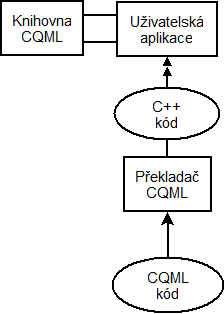
\includegraphics[width=0.7\textwidth]{Diagram1}
\caption{{\label{fig:structure1}}Návrh struktury překladače.}
\end{center}
\end{figure*}

Jedním z cílů této práce je umožnit jednoduchou rozšiřitelnost základní funkčnosti této knihovny, například přidáním dalších GUI elementů, které nebudou vycházet z funkčnosti již existujících, tudíž by to nebylo možné pouze jejich tvorbou pomocí CQML souborů. Prvky, které nejsou vytvořeny pomocí CQML souborů z již existujících prvků, se v budou nazývat vestavěné prvky.
Použití nových vestavěných typů vyžaduje jejich deklaraci v hlavičkovém souboru používaném jak v aplikaci používající knihovnu, tak i v knihovně samotné, přičemž je také nutné, aby o jejich existenci a členech věděla i aplikace překladače CQML. Aby byla rozšiřitelnost co nejjednodušší, je potřeba, aby deklarace nových prvků musela být na co nejmenším počtu míst. Z tohoto důvodu se bude deklarace nových vestavěných prvků spolu s jejich registrací pro potřeby překladače realizovat pomocí maker v jednom souboru, přičemž funkčnost těchto maker bude v jednotlivých aplikacích rozlišena pomocí konstruktů \#ifdef.
Pro usnadnění rozšiřitelnosti budou některé metody nových vestavěných prvků vygenerovány, jako například metody pro inicializaci nebo update hodnot atributů daného typu. Generování některých takovýchto metod nemusí být triviální problém, který by šlo vyřešit pomocí maker v rámci C/C++ preprocesoru. Z tohoto důvodu je nutné přidat aplikaci, která předzpracuje vestavěné typy a vypíše zdrojové kódy vygenerovaných metod, které budou použity v rámci knihovny.

\begin{figure*}[!ht]
\begin{center}
  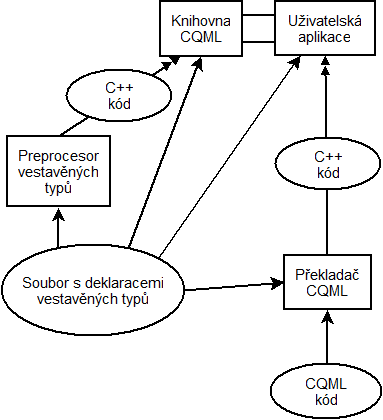
\includegraphics[width=0.7\textwidth]{Diagram2}
\caption{{\label{fig:structure2}}Návrh struktury překladače.}
\end{center}
\end{figure*}

Na obrázku \ref{fig:structure2} je ilustrován finální návrh struktury systému pro vývoj GUI v jazyce CQML. Dvojité šipky představují vztah mezi jednotlivými bloky, kde na počátku šipky je blok, na jehož výstupu je zdrojový kód, zatímco na konci šipky je blok, do kterého je zdrojový kód zahrnut. Jednoduché šipky ilustrují, do kterých bloků bude zahrnut soubor s deklaracemi vestavěných typů nebo vstup vstup CQML souborů.

\section{\label{SEC:macN}Deklarace vestavěných typů}
Jak již bylo zmíněno, deklarace nových vestavěných typů bude probíhat pomocí maker v jednom souboru. Funkčnost se bude lišit v závislosti na aplikaci, do které bude soubor zahrnut. V případě knihovny a uživatelské aplikace daná makra vygenerují pouze kód definující struktury nových datových typů. V případě překladače a preprocesoru vestavěných typů budou pomocí těchto maker volány funkce pro registraci nových datových typů spolu s funkcemi pro registraci jejich atributů. Ovšem k vygenerování kódu pomocí makra je nutné nejen makro vytvořit, ale i zajistit, že bude někdy provedeno, proto zde bude i jednoduchý seznam maker, která se mají provést. Pro účely preprocesoru a překladače bude potřeba i zaregistrovat primitivní typy, které budou moci být používány v rámci jazyka CQML, proto se v seznamu prováděných maker budou nacházet i makra pro registraci primitivních datových typů. Tato makra neprovedou nic v případě knihovny CQML či uživatelské aplikace, avšak v případě preprocesoru a překladače zavolají funkce pro registraci primitivního datového typu.

\begin{lstlisting}[frame=single,caption=Řešení v pseudokódu problematického použití operátoru "." v přiřazovacím výroku,label=lst:decprimN]
#ifdef REGISTRATION_APP
#define REGISTER_PRIMTYPE(x) RegisterPrimitive(x)
#else
#define REGISTER_PRIMTYPE(x)
#endif
\end{lstlisting}
Ve fragmentu kódu \ref{fig:decprimN} je ukázka makra, které by zavolalo funkci RegisterPrimitive s parametrem x, když je REGISTRATION\_APP definováno, přičemž neprovede nic, když  REGISTRATION\_APP definováno není.


\begin{lstlisting}[frame=single,caption=Řešení v pseudokódu problematického použití operátoru "." v přiřazovacím výroku,label=lst:decN]
#ifdef REGISTRATION_APP
#define REGISTER_STRUCTURE(macro, name) \
struct name { macro(DECL_ATTRIB) };
#else
#define REGISTER_STRUCTURE(macro, name) \
RegisterStructure(name);\
macro(REG_ATTRIB) 
#endif

#define DECL_ATTRIB(type, name) type name;

#define REG_ATTRIB(type, name) RegisterAttribute(type,name);
\end{lstlisting}
  
Fragment kódu \ref{fig:decN} ilustruje makra, která by mohla být použita pro registraci struktury v jedné aplikaci, kde je REGISTRATION\_APP definováno, a zároveň by definovali strukturu tam, kde REGISTRATION\_APP definováno není. Fragment kódu \ref{fig:decUse1N} pak ukazuje příklad použití maker, zatímco fragment \ref{fig:decUse2N} ukazuje vygenerovaný makry kód pro případ, že je REGISTRATION\_APP definováno, a fragment \ref{fig:decUse3N} pro případ opačný. Uživatel tak bude moci takovýmto způsobem přidat nový datový typ vytvořením makra pro vygenerování dané datové struktury a vložením názvu makra do seznamu prováděných maker.

\begin{lstlisting}[frame=single,caption=Řešení v pseudokódu problematického použití operátoru "." v přiřazovacím výroku,label=lst:decUse1N]
#define STRUCT_CUSTOM(OPERATION) \
OPERATION(int, first) \
OPERATION(char, second) \

REGISTER_PRIMTYPE(char)
REGISTER_PRIMTYPE(int)
REGISTER_STRUCTURE(STRUCT_CUSTOM,Custom)
\end{lstlisting}

\begin{lstlisting}[frame=single,caption=Řešení v pseudokódu problematického použití operátoru "." v přiřazovacím výroku,label=lst:decUse2N]
RegisterPrimitive(char);
RegisterPrimitive(int);

RegisterStructure(Custom);
RegisterAttribute(int, first);
RegisterAttribute(char, second);
\end{lstlisting}

\begin{lstlisting}[frame=single,caption=Řešení v pseudokódu problematického použití operátoru "." v přiřazovacím výroku,label=lst:decUse3N]
struct Custom { int first; char second; };
\end{lstlisting}
 







\section{Překladač}
Cílem je vytvořit aplikaci překladače, která přemění kód z jazyka CQML pro deklarativní GUI, kód importovatelný do aplikace v jazyce C. Tudíž na vstupu bude soubor se zdrojovým kódem v jazyce CQML a výstupem bude zdrojový kód v jazyce C, ve formě definicí datových struktur pro GUI a funkcí. Vzhledem k tomu, že jazyk C na rozdíl od vyšších programovacích jazyků (C++, Java) nepodporuje členské metody u struktur (resp. tříd), je tento nedostatek obejit tím, že se použije funkce, která je rozšířena o jeden parametr, jako který přijímá ukazatel na objekt, který by danou metodu volal. V případě virtuálních metod je jako člen struktury použit ukazatel na funkci, která se bude volat.\\
Výsledný překladač je navržen tak, že lze rozdělit do několika bloků, viz. Obrázek \ref{fig:fig1}.\\
\begin{figure*}[!ht]
\begin{center}
  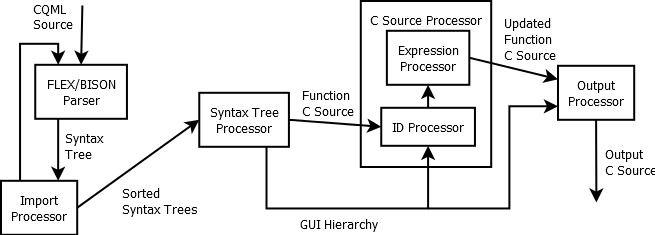
\includegraphics[width=0.7\textwidth]{parserdiag}
\caption{{\label{fig:fig1}}Návrh struktury překladače.}
\end{center}
\end{figure*}
Cílem prvního bloku (FLEX/BISON Parser) je přečíst zdrojový kód z CQML souboru a ověřit jeho syntaktickou správnost. V případě, že je kód syntakticky v pořádku, bude výstupem tohoto bloku syntaktický strom. Pro tento blok budou použity zdrojové kódy vygenerované pomocí aplikací Bison a Flex, z YACC gramatiky pro CQML.\\
V syntaktickém stromu budou nalezeny příkazy pro import souborů (blok Import Processor). Tyto soubory budou následně otevřeny a postupně zpracovány totožným způsobem.\\
Jakmile jsou všechny importované soubory zpracovány a jsou jejich zpracováním vytvořeny jejich syntaktické stromy, bude zjištěno, zda jsou některé soubory cyklicky závislé. To se bude realizovat pomocí konstrukce orientovaného grafu, kde každý vrchol představuje soubor a závislost mezi soubory je znázorněna hranou (směřující k importovanému souboru), a následným zjištěním zda v grafu existuje orientovaný cyklus. Pokud v grafu takový cyklus existuje, pak jsou soubory cyklicky závislé, což vyústí v chybu a ukončení programu. Je-li graf acyklický, jsou podle něho topologicky seřazeny syntaktické stromy jednotlivých souborů (vrcholy) pro následné zpracování.\\
V dalším bloku (Syntax Tree Processor) se zpracuje syntaktický strom a podle něj se vytvoří GUI hierarchie. Pro každý uzel představující GUI element, atribut, funkci, či nový atribut se vytvoří instance příslušné třídy. Každému elementu jsou podle jeho potomků v syntaktickém stromu přiřazeny jeho potomci v GUI hierarchii a jeho atributy a funkce.
Následně se zpracují všechny elementy s definovaným atributem ID, a tyto identifikátory se použijí ke tvorbě mapy, pomocí níž bude umožněno přistupovat k danému elementu podle definovaného identifikátoru.\\
V další části programu (C Source Processor) se zpracují kódy funkcí do formy potřebné pro závěrečný výstup v jazyce C. 

\subsection{Zpracování kódu v jazyce C}
Syntaktické stromy jednotlivých funkcí (případně výrazů) se projdou a převedou se na pole samostatných tokenů, takovým způsobem, že jeden prvek v poli bude představovat list stromu. Vzhledem k nutnosti kontroly existence atributů, budou pro snadnější zpracování některé tokeny v poli seskupeny do jednoho, který bude mít v sobě uloženo pole tokenů, které seskupil. Vzhledem k tomu, že každý token může obsahovat další tokeny, se bude stále jednat o stromovou strukturu, nicméně, bude mít nižší hloubku.\\
\begin{figure*}[!ht]
\begin{center}
  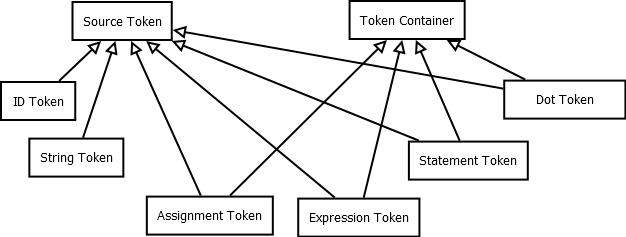
\includegraphics[width=0.7\textwidth]{tokens}
\caption{{\label{fig:fig2}}Diagram tříd tokenů.}
\end{center}
\end{figure*}

Na obrázku Obrázek \ref{fig:fig2} je znázorněn diagram tříd tokenů. Všechny tokeny dědí z jedné abstraktní třídy "Source Token". Vhledem k tomu, že pro implementaci překladače byl zvolen jazyk C++, je využito mnohonásobné dědičnosti a tokeny, jež sdružují skupinu tokenů do jednoho, dědí z třídy "Token Container". "ID Token" představuje nějaký identifikátor uvnitř kodu, zatímco "String Token" představuje jakýkoli jiný řetězec. "Dot Token" sdružuje tokeny pro výraz, v němž se pomocí operátoru "." přistupuje k atributům. "Statement Token" představuje libovolný výrok, "Assignment Token" představuje přiřazovací výraz a třída "Expression Token" libovolný jiný výraz.

\subsubsection{Zpracování identifikátorů}
Kódy (resp. syntaktické stromy) jednotlivých funkcí se projdou, a naleznou se identifikátory, jež se nachází v mapě identifikátorů elementů (id atributy elementů), a tyto identifikátory se v kódu nahradí skutečným názvem elementu uvnitř výsledné GUI aplikace.
\subsubsection{Dynamická kontrola typů a přiřazování hodnot}
Jelikož bude do atributů některých typů umožněno ukládat reference na objekty různého typu a pomocí této reference bude možné přistupovat k atributu daného objektu, nemůže být zaručeno, že atribut, ke kterému se aplikace snaží přistoupit, je v daném objektu přítomen. Proto bude potřeba za běhu výsledné GUI aplikace (využívající kód na výstupu překladače) kontrolovat přítomnost takového atributu.\\
Uvažujme kód z obrázku níže(viz.). Z kódu je zřejmé, že u atributu ref budepotřeba zkontrolovat, zda má objekt referovaný tímto atributem atribut ref2 a objekt referovaný ref2 obsahuje ref3.

\begin{lstlisting}[frame=single,caption=Pseudokód problematického použití operátoru "." v přiřazovacím výroku. ]
ref1 = ref1.ref2.ref3 = ref1.ref2.ref3
\end{lstlisting}
Oproti nahrazení identifikátoru názvem elementu nestačí pouze nahradit část textového řetězce ve výrazu. Vzhledem k tomu, že kromě ověření existence atributu bude potřeba daný atribut i získat pro další zpracování, bude nutné kód rozdělit do jednotlivých částí a každý operátor tečky nahradit voláním funkce pro získání (resp. nastavení) hodnoty atributu a kontrolou existence daného atributu.  Jak je znázorněno v kódu viz.
\begin{lstlisting}[frame=single,caption=Řešení v pseudokódu problematického použití operátoru "." v přiřazovacím výroku. ]
if(not CheckExistence(ref1, "ref2"))
	ReportException
var1 = ref1.Get("ref2");
if(not CheckExistence(var1, "ref3"))
	ReportException
var2 = var1.Get("ref3");

if(not CheckExistence(ref1, "ref2"))
	ReportException
var3 = ref1.Get("ref2");
if(not CheckExistence(var3, "ref3"))
	ReportException
var3.Set("ref3",var2);

Set("ref1",var2)
\end{lstlisting}
Díky možnosti zřetězit za sebou několik operátoru přiřazení, je potřeba rozdělit výraz na jednotlivé l-hodnoty a r-hodnoty a podle nich vybrat zda bude použit funkce pro získání nebo nastavení atributu, neboli l-hodnoty se nastaví tzv. setterem (tj. metoda pro nastavení atributu) a r-hodnoty se získají pomocí tzv. getteru (tj. metoda pro získání hodnoty atributu). Operátor "." pro přístup k atributu se zpravidla nahradí getterem, jedinou výjimku tvoří nejpravější operátor "." u nějaké l-hodnoty, neboli operátor "." nacházející se nejblíže nalevo od nějakého operátoru přiřazení.


\subsection{Výstup}
Poslední blok se postará o výpis do výstupních souborů. Pro každý zpracovaný vstupní soubor se vytvoří hlavičkový soubor s deklarací struktur a hlaviček funkcí. Každý soubor bude mít vlastní inicializační funkci pro inicializaci hierarchie a počátečnímu přiřazení hodnot a ukazatelů na potřebné funkce.\\
Pro každý GUI element, kterému je pomocí příkazu přidán nový atribut, se definuje nový typ struktury, která dědí z původního typu struktury. Každý přidaný atribut se deklaruje v nové struktuře, spolu s ukazatelem na funkci, která bude sloužit k jeho updatování. Pro každou takovou strukturu se také vytvoří funkce, které takovou strukturu alokují a inicializují, přičemž se v dané funkci zavolá funkce pro inicializaci struktury, ze které se dědí.\\
Pro všechny elementy se vytvoří funkce pro jejich update, která slouží k updatování hodnot v atributech elementů. Pro každý atribut, jemuž je přiřazena nějaká hodnota v CQML souborech, bude definována funkce pro jeho update danou hodnotou. Ukazatel na danou funkci, bude přiřazena v inicializační funkci daného souboru, do členské proměnné struktury určené pro daný atribut.\\


\section{\label{SEC:prepN}Preprocesor datových typů}
Tato aplikace bude využívat výše zmíněný soubor s deklaracemi vestavěných typů, které jsou realizovány pomocí maker (viz. sekce \ref{SEC:macN}). Pro účely předzpracování datových typů v rámci preprocesoru, se pomocí maker z daného souboru zaregistrují jednotlivé vestavěné typy, spolu se seznamem jejich atributů, a také primitivní typy. Ze seznamu atributů se vygenerují hašovací funkce pro všechny vestavěné typy pomocí algoritmu popsaného v sekci \ref{SEC:hashP}.\\
Účelem preprocesoru je vygenerovat zdrojové kódy, pro použití v runtime knihovně CQML. Vygenerují se zdrojové kódy metod pro přístup k obecnému atributu pomocí jeho jména, to k jakému atributu se bude přištupovat bude rozlišeno pomocí hodnoty haše, která je výstupem příslušné hašovací funkce. Také se vygenerují metody pro update hodnot atributů daného vestavěného typu pomocí updatovacích funkcí, které mohly být přiřazeny v rámci překladače. Dále se vygeneruje kód konstruktorů, které inicializují hodnoty atributů na jejich výchozí hodnotu, přičemž se v jejich rámci také inicializuje hodnota identifikátoru typu. Hodnota tohoto identifikátoru, který je pro každý typ unikátní, bude sloužit k výběru příslušné hašovací funkce pro daný typ v metodě pro přístup k obecnému atributu pomocí jeho jména.\\
Kód, který bude výstupem tohoto preprocesoru, bude zahrnut do kódu pro runtime knihovnu CQML.\\



\subsection {Hašování}
%Vzhledem


\section{\label{SEC:libI}Knihovna}
K zajištění co největší multiplatformní podpory CQML aplikací, bude aplikace podporovat vyměnitelný backend pro vykreslování, vstup a správu zdrojů (např. obrázky, fonty). Proto tato funkčnost nebude implementována v rámci knihovny, ale bude muset být poskytnuta v rámci uživatelské aplikace. 
Jelikož knihovna bude předkompilovaná nezávisle na uživatelské aplikaci, není možné, aby z knihovny byly přímo volány funkce v uživatelské aplikaci, protože nejsou v době kompilace knihovny ještě známy. Tudíž není možné volat například vykreslovací funkce zevnitř knihovny. Tento problém lze vyřešit předáním ukazatele na funkci v uživatelské aplikaci prostřednictvím funkce poskytované knihovnou. Vzhledem k velkému počtu vykreslovacích funkcí budou funkce sdruženy pod abstraktní třídu (interface), jako virtuální metody, které bude muset implementovat uživatelská aplikace.\\

Ve většině realtime aplikací je rozděleno vykreslování a aplikační výpočty do dvou oddělených fází, které se neprotínají. Fáze s aplikačními výpočty se zpravidla nazývá Update. Tyto fáze jsou tudíž odděleny i v případě knihovny. Během vykreslovací fáze bude vykreslována aktuální GUI hierarchie, zatímco během fáze Update se budou přepočítávat hodnoty uvnitř jednotlivých elementů.\\

\subsection {Vstup}
V realtime aplikacích se v některých případech bere vstup ze vstupních zařízení v odděleném vláknu, než v jakém probíhá hlavní vlánko aplikace, to má za úkol zajistit, že aplikace nezamrzne vůči uživatelově vstupu v případě, že právě provádí složitý výpočet či vykresluje složitý obraz. Proto bude knihovna podporovat tento přístup. Vstup bude zpracovávat pomocí událostí, události bude muset generovat uživatelská aplikace, která je bude prostřednictvím funkce ukládat do fronty pro jejich zpracování. Vkládat události do fronty bude umožněno i v odděleném vláknu, proto bude knihovna využívat threadsafe frontu, která bude realizována pomocí dvou oddělených front, přičemž do jedné fronty bude možno vkládat události, zatímco se druhá bude zpracovávat (viz. obrázek \ref{fig:que1N}). Zpracování fronty bude probíhat na počátku fáze Update, jakmile se fronta zpracuje, prohodí se fronta pro vkládání událostí a pro zpracování. Fronta bude pomocí vláknových zámků zajišťovat, že při vkládání zároveň s prohozením front, nebo při vkládání událostí ze dvou vláken v tentýž okamžik, nedojde k porušení atomicity jednotlivých operací.\\

\begin{figure*}[!ht]
\begin{center}
  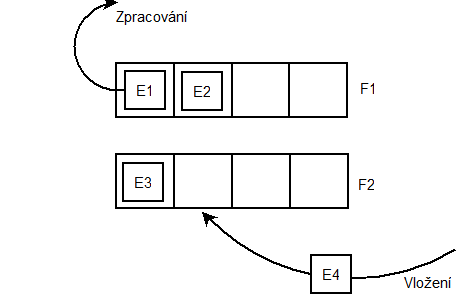
\includegraphics[width=0.7\textwidth]{Diagram5}
\caption{{\label{fig:que1N}}Návrh realizace fronty.}
\end{center}
\end{figure*}

Komunikace mezi knihovnou a uživatelskou aplikací je ilustrována na obrázku \ref{fig:lib1N}.\\


\begin{figure*}[!ht]
\begin{center}
  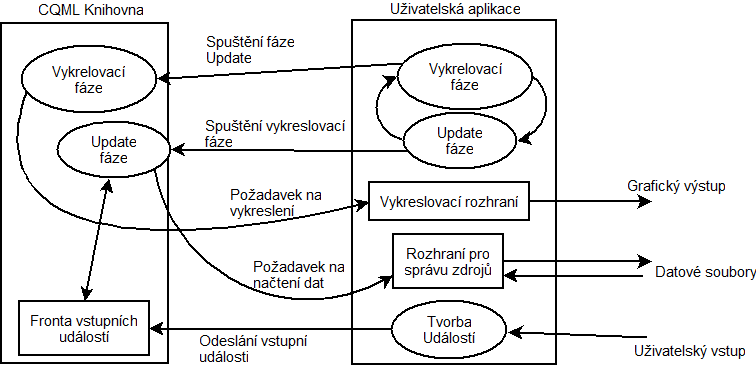
\includegraphics[width=0.7\textwidth]{Diagram4}
\caption{{\label{fig:lib1N}} Návrh komunikace mezi knihovnou }
\end{center}
\end{figure*}

\subsection {Správa GUI}
Hierarchie vygenerovaného GUI bude uchovávána v podobě stromu. Na vrcholu stromu se tudíž nachází kořenový element, jež může mít teoreticky neomezený počet potomků, přičemž každý takovýto potomek je element, který může mít opět neomezený počet potomků. Každý vestavěný datový typ, který bude přímo součástí hierachie a ne pouze atributem nějakého elementu, bude dědit z obecné struktury Element. Každý uzel v rámci stromu GUI, tak bude typu Element nebo typu, který je z něj odvozen. Typ Element bude struktura, která bude obsahovat pole jeho potomků, atributy souřadnice a velikost. Struktura Element bude vlastnit virtuální metody Draw a Update, které budou moci struktury z nich odvozené přetěžovat.
%-- element

Každý element může mít atributy, které budou přístupné zevnitř jazyka CQML. Takové atributy uvnitř struktury reprezentující daný element, nejsou představovány pouze členem pro uchování jejich hodnoty, ale také ukazatelem na funkci, která může slouží k přepočítání hodnoty daného atributu v rámci fáze Update. Funkce, na kterou daný ukazatel ukazuje, je vygenerována v pomocí překladače a je danému atributu přiřazena, uvnitř kódu vygenerovaném překladačem. Jelikož se jedná o ukazatel na funkci a nikoliv o metodu samotného elementu, je uchováván i tzv. kontext funkce. Kontextem funkce je v tomto případě myšlen CQML soubor v jehož rámci byla daná funkce specifikována, což znamená, že tato funkce by měla být schopna přistupovat ke všem prvkům specifikovaných v daném souboru. Jelikož každý CQML soubor představuje samostatnou komponentu, je tak kontext uložen ve formě struktury, která obsahuje ukazatel na kořenový prvek v rámci dané komponenty (souboru) a také ukazatel na element jemuž byla funkce s daným kontextem uložena.
%--
Každý element v GUI hierarchii má metodu Update, kterou dědí z typu Element. Tato metoda má za úkol přepočítat hodnoty atributů, jsou-li jim přiřazeny funkce pro jejich přepočítání. Dále tato metoda zavolá Update všech potomků daného elementu.

\subsection {Vykreslování}
Aby bylo zajištěno, že se prvek nacházející se výše v hierarchii vždy vykreslí před prvky jež jsou v hierarchii níže, tak se pro vykreslování použije fronta. Na počátku vykreslovací fáze se do ní zařadí pouze prvek na vrcholu hierarchie. Na prvek ve frontě se zavolá jeho vykreslovací metoda, která jej vykreslí a záriveň přidá jeho potomky na konec fronty. Po vyprázdnění fronty se ukončí fáze vykreslování.
Jak již bylo zmíněno, samotné vykresovací funkce budou z knihovny pouze volány pomocí vykreslovacího rozhraní poskytovaného uživatelskou aplikací. Tyto funkce budou volány zevnitř přetížených metod Draw, jednotlivých elementů. Každý vestavěný typ, který dědí z typu Element může přetěžovat vykreslovací metodu Draw.\\


Jelikož by knihovna CQML měla umožnit použití externích zdrojů, jako jsou například obrázky či fonty, v obecném formátu. Bude správa těchto dat obsluhována uvnitř uživatelské aplikace podobně, jako je tomu u vykreslování, pomocí speciálního rozhraní. Každý element, který taková data vyžaduje bude moci v rámci své přetížené metody Update dát do fronty požadavek pro načtení dat.\\
Tyto požadavky budou zpracovány na konci fáze Update zavoláním příslušné metody rozhraní pro načtení dat. Metody rozhraní budou vracet hodnotu typu void*, což může představovat ukazatel na libovolná data. Tato hodnota, pak bude uložena do mapy, pod specifickým identifikátorem, v případě obrázku bude takovým identifkátorem název souboru, v případě fontu bude tento identifikátor název fontu, který bude mít za sebou připojeny parametry fontu ve formě textového řetězce. Kdykoliv pak bude knihovna vyžadovat manipulaci s externím zdrojem (například předáním funkci pro vykreslení), učiní tak pomocí dané hodnoty typu void*. \\

\subsection {Hašování}

\subsection {Inicializace}
Před použitím CQML knihovny v rámci uživatelské aplikace bude nutné knihovnu nejprve inicializovat. Během inicializace bude nutné knihovně předat ukazatele na instance objektů rozhranní jež budou složit ke správě externích zdrojů a vykreslování. Také bude potřeba předat knihovně ukazatel na funkci pro inicializaci Hašovacích funkcí.\\




\subsection {Variant}
Některé atributy některých elementů mohou být typu reference na element, který mohl být rozšířen o atribut libovolného typu a názvu. Jelikož se element, na který daná reference ukazuje, může změnit za běhu, nelze staticky určit typ atributů referovaného element. Z tohoto důvodu bude k atributům takového elementu nutno přistupovat pomocí virtuální metody, která musí vracet nějaký obecný typ, do kterého může být uložena hodnota libovolného typu, se kterou bude následně možno manipulovat uniformním způsobem.\\
Pro manipulaci s hodnotami různého datového typu uniformní způsobem lze v jazyce C/C++ použít konstrukt union. Konstrukt union však nelze použít v objektově orientovaném prostředí, jelikož nepodporuje použití datových typů s netriviálním konstruktorem či destruktorem, datové typy s triviálním konstruktorem se označují zkratkou POD, neboli "Plain old data" (v doslovném překladu "Prostá stará data").\\
Pro jazyk C/C++ existuje knihovna Boost, která poskytuje řešení v podobě šablony variant. Šablona variant umožňuje uložení libovolného datového typu, ať už se jedná o typ POD či nikoliv.\\
V jazyce QML tuto funkci má datový typ var. Tento typ má obdobnou funkci jako proměnná v jazyce JavaScript, tudíž je do něj možné uložit data libovolného datového typu. Proměnný typ var tak umožňuje nejen ukládání primitivních a složených datových typů, ale lze také použít k uložení referencí na grafické elementy. Tento typ také podporuje provádění aritmetických operací, uložení do jiné proměnné libovolného typu, přičemž pokud dojde k použití aritmetické operace mezi nekompatibilními typy, či pokusu o uložení do proměnné nekompatibilního typu, pak QML aplikace vyhodí výjimku.\\
Pro účely knihovny CQML je tedy vhodné vytvořit datový typ, který by se svou funkčností co nejvíce podobal typu var jazyka QML. Tento typ bude nazýván Variant. Pro odlišení mezi šablonou variant poskytovanou knihovnou boost má název tohoto typu velké počáteční písmeno.\\
Typ Variant v knihovně CQML bude přetěžovat operátory aritmetických operací a operátor přiřazení. Typ Variant bude podporovat konverzi na libovolný datový typ pomocí metody As, která bude definována pomocí šablony, jenž bude přijímat požadovaný datový typ jako parametr. Typ Variant bude uchovávat identifikátor svého typu a svou hodnotu. Za účelem, aby se každá operace prováděla jen mezi totožnými typy, bude zavedena konvence, že při použití binárního operátoru bude vždy pravý operand přetypován na typ levého operandu. Každá konvenrze mezi typy, které nejsou kompatibilní (například mezi nečíselným a číselným typem) vyústí v chybu.\\
Typ Variant bude podporovat metodu Get, podobně jako ostatní typy používané v rámci knihovny CQML. V případě, že je v typu Variant uložen primitivní typ, který nemá žádné atributy, pak dojde k ohlášení chyby, podobně jako by tomu bylo v případě žádosti o získání neexistujícího atributu.\\

Při manipulaci s atributy elementu referencovaného nějakým atributem jiného elementu může dojít k situaci, kdy je potřeba hodnotu referencovaného atributu změnit (viz. k). Problémem, který zde nastává je, že metoda Get vrací hodnotu typu Variant, která není nijak vázaná na adresu, kde byla původní hodnota uložena. Proto je potřeba vytvořit další datový typ, který narozdíl od typu Variant bude namísto hodnoty uchovávat adresu, kde byla původní hodnota uložena. Tento datový typ budiž nazván VariantRef. VariantRef bude implementovat metodu Get, stejně jako ostatní typy používané v rámci CQML. VariantRef bude také přetěžovat operátor přiřazení, přičemž při použití tohoto operátoru se změní hodnota na adrese, na níž VariantRef ukazuje. Kvůli možnosti změnit hodnotu referencovaného atributu budou tedy metody Get všech typů v řámci CQML (včetně VariantRef a Variant) vracet typ VariantRef namísto Variant. Jelikož typ Variant podporuje narozdíl od VariantRef i aritmetické operace, bude VariantRef podporovat implicitní přetypování na typ Variant, zkopírováním hodnoty na adrese, na níž ukazuje VariantRef, do nové instance typu Variant.\\


\begin{lstlisting}[frame=single,caption=Řešení v pseudokódu problematického použití operátoru "." v přiřazovacím výroku,label=lst:var1N]
reference1.att1 = reference2.att2 = reference3.att3 + 3;
\end{lstlisting}

\begin{lstlisting}[frame=single,caption=Řešení v pseudokódu problematického použití operátoru "." v přiřazovacím výroku,label=lst:var2N]
reference1.Get("att1") = reference2.Get("att2") = reference3.Get("att3") + 3;
\end{lstlisting}
Fragment \ref{lst:var2N} ukazuje, jak by vypadal kód funkce z fragmentu \ref{lst:var1N} po přeložení do C++. Výsledky metod Get jsou hodnoty typu VariantRef, přičemž výsledek operace sčítání v daném kódu bude typu Variant. Tudíž se změní hodnota attributu att1 v prvku referencovaném v reference1 a hodnota atributu att2 v prvku referencovaném v reference2.\\

\section{\label{SEC:aa}Překladač}




\part{\label{CH:aa}Implementace}

\section{\label{SEC:aa}Překladač}
\subsection{Zpracování vstupu}
Pomocí generátoru Bison byl podle gramatiky jazyka CQML vytvořen parser. Pro vygenerování lexikálního analyzátoru byl použit FLEX. Zdrojový kód parseru a lexikálního analyzátoru je pak použit v překladači.
Po spuštění program načte výchozí typy GUI elementů, uloží si jejich názvy a seznam jejich atributů, včetně jejich typů a výchozích hodnot, do instancí třídy "ClassContainer".\\
Program na vstupu přijímá jméno souboru, se zdrojovým kódem v jazyce CQML. Pokud daný soubor existuje, je otevřen a jeho obsah je předán parseru. Pokud parser detekuje syntaktickou chybu ve zdrojovém souboru, vypíše chybu a program se ukončí. Výstupem parseru je syntaktický strom. V první fázi se ve stromu vyhledají příkazy pro import elementu z jiných souborů. Totéž program cyklicky provede pro všechny soubory, z nichž se elementy importují.

\subsection{Konstrukce a zpracování pomocných struktur}
Následně je vytvořen orientovaný graf vzájemných závislostí mezi jednotlivými soubory, kde každý vrchol představuje soubor a každá hrana představuje vazbu mezi soubory, zatímco počátečním vrcholem hrany je vrchol představující soubor, do něhož je element importován, a koncovým vrcholem je vrchol představující soubor, z nějž byl element importován. Pomocí algoritmu prohledávání do hloubky je zjištěno, zda se v grafu nachází cyklus. Pokud se v grafu nachází cyklus, je vypsána chybová hláška a program se ukončí.\\
Jelikož je graf acyklický, pak každý vrchol představuje komponentu a tak lze jednotlivé vrcholy grafu a tudíž i soubory topologicky seřadit. Soubory (resp. vrcholy v grafu) jsou seřazeny pomocí Tarjanova algoritmu. Syntaktické stromy jednotlivých seřazených souborů jsou postupně zpracovány následujícím způsobem.\\
Během průchodu stromem se postupně alokují instance třídy Element, přičemž každá instance představuje určitý element v hierarchii GUI. Každému elementu je přiřazen jeho typ a seznam jeho potomků resp. elementů, které se v hierarchii nachází níže. Dále je každému elementu, u nějž jsou definované změny některých z jejich atributů, přiřazena množina dvojic názvů atributů a jejich hodnot. Hodnotou v tomto případě nemusí být konstanta, ale i výraz v jazyce C, jehož výpočtem se získá daná hodnota ve vygenerovaném zdrojovém kódu. Atributu může být také přiřazen kód celé funkce nejen samostatný výraz, v tomto případě by daná funkce vracela hodnotu atributu. Kód v jazyce C je ve formě syntaktického stromu předán funkci "SourceToHandler" (jedná-li se o celou funkci) nebo "ExpressionToHandler" (jedná-li se pouze o výraz). Výstupem obou funkcí je instance třídy "SourceHandler", která zdrojový kód v podobě posloupnosti tokenů, způsobem popsaným v kapitole (viz.). V tomto případě není tokenem myšlen pouze symbol či řetězec v syntaktickém stromu, jenž je výstupem parseru, ale i struktura obsahující pomocná data (např. informace o tom zda bude token nahrazen něčím jiným).\\
Dále program vytvoří mapu identifikátorů, pro všechny elementy, u nichž byl nastaven atribut "id". Tento atribut musí mít unikátní hodnotu, pokud je v souboru více než jeden element nastaven na stejnou hodnotu atributu "id", dojde k chybě. Pro každý soubor se uchovává jedna mapa identifikátorů.\\
Každému elementu je podle jeho specifikovaného typu přiřazen ukazatel na instanci "ClassContainer". Pokud byly nějakému elementu přiřazeny nové atributy (pomocí klíčového slova property), bude muset být ve výstupním kódu daný element reprezentován speciální třídou, tudíž se vytvoří nová instance "ClassContainer", do které jsou mimo výchozích atributů přidány i atributy nové. Všechny nové atributy musí být buď nějakého výchozího typu, nebo musí typem nějakého importovaného či výchozího elementu, jinak dojde k chybě.

\subsection{Zpracování kódu v jazyce C}
Vzhledem k tomu, že se lze v částech, které jsou napsané v jazyce C, odkazovat na jiné elementy pomocí jejich identifikátorů "id", je nutné analyzovat výrazy a nahradit ve výsledném kódu identifikátory referencemi na dané elementy. To je vyřešeno projitím všech tokenů, jež obsahují identifikátor, a vyhledáním příslušného identifikátoru v mapě identifikátorů (pro právě zpracovávaný soubor). Je-li identifikátor nalezen, pak se k příslušnému tokenu zapíše, že má být ve výstupu nahrazen referencí na identifikovaný element.\\
Následně se v kódu zpracují všechny operátory "." pro přístup k atributu tak, že se každý takový operátor nahradí voláním funkce pro nastavení nebo získání hodnoty atributu. V případě, že se operátor "." nachází nejblíže nalevo od operátoru přiřazení, nahradí se funkcí pro nastavení (setterm), v opačném případě funkcí pro získání hodnoty (getterem), jako je tomu (viz.). Pro ukládání výsledků těchto funkcí se používají pomocné proměnné. Vzhledem k tomu, že se mohou tyto operátory nacházet uvnitř výrazů, je celý řetězec operátorů "." nahrazen až názvem proměnné, ve které je uložen výsledek posledního z nich a volání funkcí, jež jejich funkčnost nahrazuje, se připojí před začátek výroku, ve kterém se nachází. Začátek výroku je symbolizován specifickým tokenem, a tudíž se volání funkcí připojí k němu v podobě datové struktury udávající typ funkce a jména pomocných proměnných, což bude použito při generování výstupu.

\subsection {Hašování}

\subsection{Výstup}
Na závěr jsou pro každý zpracovaný soubor vytvořeny tři výstupní soubory, jejichž názvy jsou zakončeny ".h", ".c", "outer.h". 
Do prvního souboru ("*.h") jsou zapsány hlavičky konstruktorů hlavní komponenty a také definice této komponenty, respektive struktury, jenž ji reprezentuje, tudíž se do těla struktury vypíší členské proměnné (reprezentujících GUI elementy v komponeně). Pro každý nový typ definovaný ve zpracovávaném souboru (reprezentovaný instancí třídy "ClassContainer") se vytvoří totéž, přičemž do těla struktury se jako členské proměnné vypíší atributy třídy, avšak první členskou proměnnou bude proměnná typu struktury, jenž představuje element, z něhož tento nový element vychází (tímto se realizuje dědičnost v jazyce C).\\
Do druhého souboru ("*.c") jsou zapsány definice všech vygenerovaných funkcí. Každý atribut má také přidělenou funkci, která se stará o jeho update. Struktura obsahující atribut obsahuje i ukazatel na danou funkci. Do těla takové funkce je zapsán kód výrazu nebo funkce, přiřazený danému atributu v CQML souboru, který byl upraven a nyní je uložen v instanci třídy "SourceHandler" příslušící danému atributu.\\
Každá struktura má definovány dva konstruktory, jeden inicializuje instanci struktury, přiřadí každému atributu počáteční hodnotu a všem ukazatelům na funkce příslušnou funkci, a druhý alokuje paměť pro danou strukturu a poté zavolá první konstruktor. Jelikož jazyk C nepodporuje konstruktory struktur, je zde pojmem konstruktor myšlena funkce pro vytvoření instance struktury.\\
Do třetího souboru ("*outer.h") jsou jsou zapsány pouze hlavička konstruktoru hlavní komponenty souboru a deklarace struktury představující hlavní komponentu. Tento soubor slouží k začlenění do souboru, jež danou komponentu bude používat.\\
Jakmile jsou takto zpracovány všechny vstupní soubory, vytvoří se poslední výstupní soubor, ve kterém se definuje hlavní inicializační funkce, ve které se vytvoří instance hlavní komponenty GUI (komponenta prvního souboru, který byl programu zadán), a také funkce pro volající update této komponenty.\\

\section{\label{SEC:macI}Přidávání vestavěných typů}
Vestavěné struktury lze rozdělit na dvě různé skupiny. První skupina jsou struktury, ke kterým se bude v rámci aplikace přistupovat jako k referenčním typům, tudíž při manipulaci s nimi se manipuluje s referencí ukazující na jejich umístění v paměti. Ve druhé skupině jsou struktury, které fungují jako hodnotové typy, takže se manipuluje přímo s jejich obsahem.\\


Zdrojový kód je sdílený mezi několika aplikacemi. Pomocí konstruktu \#ifdef CQML\_PARSER je rozlišeno, jaké definice maker se budou v dané aplikaci používatW. Přičemž makro CQML\_PARSER je definováno pro aplikaci překladače a preprocesoru vestavěných typů, zatímco pro grafickou knihovnu a uživatelskou aplikaci definováno není. Výstupem jsou tedy dvě verze kódu. Verze s definovaným makrem CQML\_PARSER bude dále označována jako parser verze. Verze bez definice makra CQML\_PARSER bude dále označována jako runtime verze.\\

Prvním makrem je makro REGISTRATION, toto makro je jedinné voláno přímo, zatímco ostatní makra pro definici vestavěných datových typů jsou volána prostřednictvím tohoto makrem ať už přímo nebo transitivně. Makro REGISTRATION se v parser verzi nachází uvnitř funkce RegisterBasicTypes(), která je volána na začátku aplikací překladače a preprocesoru vestavěných typ. V runtime verzi se toto makro nachází uvnitř namespace CQML\_GUI. Makro samotné v obou verzích má totožnou funkčnost. REGISTRATION přijímá tři parametry, jimiž jsou makra. První je reprezentováno názvem MACRO2, které slouží pro registraci nové struktury hodnotového typu, zatímco druhým parametrem je MACRO2REF, které slouží pro registraci struktury referenčního typu. Třetím parametrem je MACRO3, což slouží pro registraci struktury dědící z jiného již registrovaného datového typu. MACRO2 a MACRO2REF přijímá jako první parametr název makra pro generování datové struktury, jako druhý parametr přijímá název datové struktury. MACRO3 má totožné první dva parametry, ale má i třetí parametr, který je názvem datového typu, ze kterého generovaná struktura dědí. \\
Na počátku makra REGISTRATION se volají makra REGPRIMITIVE pro primitivní datové typy, jako jsou například int, char či float. V parser verzi se pomocí makra REGPRIMITIVE zavolá funkce RegisterPrimitive, která jako parametr přijímá název primitivního datového typu, který byl makru předán jako parametr. Makro REGPRIMITIVE v případě runtime verze neprovede nic. Ve zbytku makra REGISTRATION se volají makra, která mu byla předána v parametrech, s parametry pro registraci jednotlivých datových typů.\\
Makru REGISTRATION jsou v runtime verzi předána makra MAKE\_STRUCTURE2 (toto makro je předáno jako první dva parametry) a makro MAKE\_STRUCTURE3. Zatímco v parser verzi jsou předána makra PARSER\_DECLARE2, PARSER\_DECLARE2REF a PARSER\_DECLARE3.\\
Makra MAKE\_STRUCTURE2 a MAKE\_STRUCTURE3, mají téměř totožnou funkčnost. Vytvoří tělo struktury s definovaným názvem, konstruktorem a metodou Get pro získání libovolného atributu. Jedinným rozdílem je, že v případě makra MAKE\_STRUCTURE3 dědí vygenerovaná struktura z typu, jehož název byl makru předán pomocí třetího parametru, zatímco struktura vygenerovaná makrem MAKE\_STRUCTURE2 dědí ze struktury CQMLObject. Makro, které bylo předáno jako první parametr, slouží k vygenerování kódu pro deklaraci atributů v těle dané struktury, pomocí maker několika maker, jež mu jsou předány jako parametry.\\
%..

Makra PARSER\_DECLARE2, PARSER\_DECLARE2REF a PARSER\_DECLARE3, volají funkci, které jako první parametr předají jméno struktury (druhý parametr předaný makru) a jako druhý parametr předají nulu, v případě prvních dvou maker, a v případě třetího makra se předá jméno rodiče (třetí parametr předaný makru). První a třetí makro takto volá funkci RegisterStruct a druhé makro takto volá funkci RegisterStructRef. Všechny tři makra na závěr zavolají makro, jenž jim bylo předáno prostřednictvím prvního parametru. Volané makro slouží k zavolání funkcí pro registraci jednotlivých atributů, pomocí několika maker, jež mu jsou předány jako parametry.\\
%..

Zmíněná makra PARSER\_DECLARE2, PARSER\_DECLARE2REF, PARSER\_DECLARE3, MAKE\_STRUCTURE2 a MAKE\_STRUCTURE3 příjímají jako první parametr stejný druh makra, respektive makra vycházející ze stejného vzoru. Toto makro slouží pro vygenerování deklarace atributů v runtime verzi a pro registraci atributů v parser verzi. Pro každý vestavěný typ je jedno takové makro. Makro přijímá 5 maker jako a svoje parametry v následujícím pořadí.\\
\begin{description}
\item[MF] slouží pro vytvoření atributu, který bude přístupný pouze ve vnitřním C++ kódu knihovny. V parser verzi toto makro zaregistruje daný atribut. V runtime verzi toto makro deklaruje atribut uvnitř struktury.
\item[F] slouží pro vytvoření atributu, který bude přístupný uvnitř CQML souborů i ve vnitřním C++ kódu knihovny. V parser verzi toto makro zaregistruje daný atribut. V runtime verzi toto makro deklaruje atribut uvnitř knihovny, spolu s ukazatelem na funkci pro jeho výpočet a ukazatelem na kontext, v jakém bude daná funkce  operovat.
\item[M] vytvoří ukazatel na funkci, která může sloužit například k obsluze událostí. V parser verzi toto makro zaregistruje daný ukazatel. V runtime verzi toto makro deklaruje ukazatel na funkci spolu s ukazatelem na kontext, v jakém bude daná funkce operovat. 
\item[ME] deklaruje metodu, kterou bude nutno implementovat v rámci zdrojového kódu knihovny. V parser verzi toto makro neprovede nic. V runtime verzi deklaruje hlavičku metody.
\item[MEV] deklaruje virtuální metodu, kterou bude nutno implementovat v rámci zdrojového kódu knihovny. V parser verzi toto makro neprovede nic. V runtime verzi deklaruje hlavičku virtuální metody.
\end{description}

Všechna uvedená makra přijímají jako první parametr typ (v případě metod a ukazatelů na funkce je to návratový typ), jako druhý parametr název, jako třetí parametr výchozí hodnotu (tento parametr je irelevantní pro metody). Makra M, ME a MEV přijímají jako zbylé parametry seznam parametrů daných funkcí (resp. metod).\\

%.. příklad


\section{\label{SEC:aa}Preprocesor vestavěných typů}
\subsection{Inicializace}
Na počátku programu jsou spuštěny funkce pro registraci vestavěných typů a podporovaných primitivních typů, volání těchto funkcí jsou vygenerovány prostřednictvím maker (viz. sekce \ref{SEC:macI}).\\
Registrované typy jsou uloženy do dvou polí, přičemž jedno pole obsahuje seznam jmen primitivních datových typů, a druhé pole obsahuje struktury uchovávající data o vestavěných typech. Každému vestavěnému typu jsou přiřazeny atributy, které budou přístupné z CQML kódu, atributy, které budou přístupné pouze z C++ kódu, a také ukazatele na funkce, jenž budou sloužit k obsluze událostí. Jednotlivým atributům je přiřazen jejich typ, jméno a výchozí hodnota. Pro každý zaregistrovaný vestavěný typ je postupně vygenerována hašovací funkce viz.. Specifika této funkce jsou uložena do instancí třídy PerfectHashData. \\
%.. perfect hash data


\subsection{Generování výstupního kódu}
V další části preprocesorové aplikace jsou vygenerovány zdrojové kódy pro použití v runtime knihovně CQML.
Nejprve se pro každý vestavěný typ vygeneruje zdrojový kód konstruktoru. Ve kterém se každému z jeho atributů přiřadí jeho výchozí hodnota. Každý vestavěný prvek má atribut typu integer s názvem classID, do nějž se ve vygenerovaném kódu přiřadí identifikátor třídy, v tomto případě je identifikátorem třídy číslo označující pořadí, v jakém byl daný vestavěný typ zaregistrován.\\
%///insert obr.
Následně je zapsán kód metody Get, pro získání libovolného atributu daného elementu, která na vstupu přijímá řetězec a jejíž návratovou hodnotou je typ VariantRef.\\
Na počátku této vygenerované metody, se zavolá funkce GetHash, které je předána hodnota parametru classID a vstupní řetězec. Tato funkce vybere z pole funkcí pomocí hodnoty classID hašovací funkcí, pomocí níž spočte hodnotu haš pro vstupní řetězec. Hodnota haš je předána konstruktu switch. V konstruktu switch je každé větvi case dána hodnota pro haš představující určitý atribut (spočtená předáním jména atributu příslušné hašovací funkci), v takovém případě daná funkce vrátí referenci na daný atribut ve formě datového typu VariantRef. Pokud hodnota předaná konstruktu switch nesouhlasí s hašem žádného atributu, pak mocí větve default vyhodí program výjimku.\\

%/// insert příklad a details

V poslední části generování zdrojových kódů v rámci preprocesoru, jsou vygenerovány zdrojové kódy metody Update pro každý vestavěný prvek. Metoda Update je vygenerována pouze pro vestavěné referenční typy, pro hodnotové typy tomu tak není. \\
Pro každý atribut, který je buď primitivního typu, nebo se jedná o vestavěný referenční typ, je do kódu této metody vložen konstrukt if, který se táže, zda má daný atribut přiřazen ukazatel na funkci pro update daného atributu, která jeho hodnotu znovu přepočítá, pokud ano, pak se daná funkce zavolá.
Pokud se jedná o atribut vestavěného hodnotového typu, pak se provede totéž, s tím rozdílem, že za if je vložen konstrukt else, v němž se nachází další konstrukty if, které se dotazují na atributy uvnitř daného atributu stejným způsobem. Tudíž v případě, že není danému atributu přiřazen ukazatel na funkci pro jeho update, pak se funkce dotáže, zda totéž platí pro jednotlivé podatributy daného atributu a případně (jsou-li přiřazeny) je zavolá.\\


\section{\label{SEC:aa}Knihovna}


\subsection{Inicializace}
Inicializace má několik fází. Nejprve je nutné zavolat funkci \_CQML\_Init(), která zavoláním funkcí MakeQueue() a InitQueueThreadsafe() vytvoří a inicializuje frontu pro vstupní události. V rámci
V další fázi inicializace je potřeba knihovně předat instance tříd implementující rozhraní pro vykreslování a správu externích zdrojů. Což je učiněno zavoláním funkcí SetDrawIFace, pro vykreslování, a SetResourceManager, pro správu externích zdrojů.
Na závěr inicializace se zavolá funkce \_CQML\_Start, která je vygenerována v překladači a provede následující úkony.
Pomocí funkce SetInitHashTabs, přijímá jako parametr ukazatel na funkci, je uložen do proměnné ukazatel na funkci pro inicializaci hašovacích funkcí. Inicializace hašovacích tabulek je následně provedena, když funkce CQMLInitHashes zavolá funkci uloženou v proměnné nastavené pomocí SetInitHashTabs.
Pomocí funkce SetRoot je knihovně předán kořenový prvek hierarchie. Na závěr inicializace se zavolá funce \_CQML\_Update(), pro inicializaci atributů GUI na validní hodnoty.	

\subsection{Update}
%Update
Funkce \_CQML\_Update() zavolá metodu nejprve funkci PreUpdate(), která spustí zpracování fronty vstupních událostí (viz. zpracování). Následně zavolá funkci Update kořenového prvku. Na závěr je zavolána funkce PostUpdate(), která se postará o načtení externích zdrojů prostřednictvím rozhraní pro jejich správu (viz. zpracování).\\
Každý element v GUI hierarchii dědí ze základního typu Element ať již přímo či transitivně, přičemž překrývá jeho metodu Update. Metoda Update každého odvozeného elementu je vygenerována buď v rámci preprocesoru vestavěných typů (pro vestavěné typy) nebo v rámci překladače (pro typy definované pomocí CQML). Každá vygenerovaná metoda volá metodu DefaultUpdate, která může, ale nemusí, být překryta, přičemž slouží k implementaci další funkčnosti v rámci Update fáze, kterou vygenerovaný kód neposkytuje. Na závěr metody Update se zavolá metoda Update nadřazené třídy (resp. struktury), s výjimkou metody Update poskytované v rámci struktury Element.\\

\subsection{Vykreslování}
Během vykreslovací fáze se zavolá metoda kořenového elementu, která vykreslí daný element a vloží všechny jeho potomky na konec vykreslovací fronty. Následně se odebere přední element z fronty a zavolá se jeho vykreslovací metoda, která jej vykreslí a vloží jeho potomky na konec fronty. To pokračuje, dokud se nevykreslí všechny GUI elementy ve stromové struktuře a fronta není prázdná.\\
%Každý element, který překryje původní vykreslovací funkci 
Veškerá funkčnost pro vykreslování na obrazovku je realizováno prostřednictvím vykreslovacího rozhraní DrawIFace.\\


\subsection{Zpracování vstupu}
Knihovna přijímá vstup ve formě událostí, které jsou vkládány do fronty pro zpracování. Fronta pro zpracování je realizována pomocí zámků realizována jako threadsafe. .. \\
Což znamená, že pro případ použití ve vícevláknové aplikaci nehrozí, že dojde k problémům, způsobených tím, že více vláken přistupuje k této frontě najednou.
Na počátku fáze Update se zavolá funkce ProcessEvents, která má za úkol zpracovat události ve vstupní frontě. Během zpracování jednotlivých událostí se každá událost vybere z fronty, následně se každá událost pošle kořenovému elementu ke zpracování, pokud ji element není schopen zpracovat sám, je událost přeposlána jeho potomkům, tatáž operace se opakuje i pro potomky, dokud se nenarazí na element schopný zpracování události nebo nejsou vyčerpány všechny elementy.\\
%// implementace konkrétních atp.


\subsection{Správa externích zdrojů}
Ve fázi Update jednotlivých elementů, se mohli změnit adresy nebo parametry některých elementů používajících externí zdroje, tudíž může být nutné některé zdroje načíst znovu. Proto se u všech elementů, u kterých k tomuto mohlo dojít, uloží do fronty požadavek pro načtení daného externího zdroje. Požadavek je ve formě textového řetězce, který jej přesně specifikuje.\\
%	Deteaily
V další fázi se zpracují všechny požadavky ve frontě. Načtená data jsou v rámci kódu knihovny uchovávána v mapě, která jako klíč pro záznam používá textový řetězec požadavku a jako data záznamu je v ní obecný ukazatel typu void* ukazující na data načtená data externího zdroje. V případě, že již byl načten totožný požadavek v minulosti, pak se nebude načítat znovu. To je rozpoznáno tak, že se v mapě již nachází záznam pod daným klíčem. V opačném případě, se prostřednictvím ifacu… Zavolá funkce pro načtení daného externího zdroje … Data jsou pod klíčem v podobě řetězce uložena do mapy.\\
Kdykoli pak knihovna potřebuje předat uživatelské aplikaci data načtená z externího zdroje, učiní tak předáním void* ukazatele uloženého v mapě.\\

\subsection{Datový typ Variant}
Každý typ používaný v rámci CQML s výjimkou primitivních, implementuje metodu Get, která jako parametr přijímá název atributu, který by měl být členem dané struktury. Tato metoda vrátí hodnotu daného Atributu převedenou na typ Variant.\\
Součástí typu Variant je identifikátor typu hodnoty, jaká je uvnitř dané instance uchovávána. Samotnou hodnotu uchovává pomocí konstruktu union, jež obsahuje jeden atribut pro každý datový typ, který je možné v typu Variant uchovávat. Jelikož v rámci konstruktu union, nelze uchovávat datové typy s netriviálním konstruktorem, jsou takové typy uchovávány pomocí ukazatele, přičemž jejich hodnota je do typu Variant uložena zkopírováním na alokované místo na haldě, a uložením ukazatele na dané místo v paměti.\\

Variant umožňuje pomocí metody As získat hodnotu uloženou v dané instanci, převedenou do libovolného kompatibilního typu. V případě, že se nejedná o převod mezi kompatibilními typy, například se z nečíselného typu pokusí převést na číselný, dojde k chybě a vyhození výjimky.  Metoda As je implementována pomocí šablony, jejímž parametrem je typ, který má metoda vracet.\\
%// příklad
Variant podporuje základní aritmetické operace, které implementuje prostřednictvím přetíženého operátoru. 
Při použití binárních operátorů mezi typy, jež nejsou totožné, dojde k převodu pravého operandu na typ levého operandu, pomocí metody As, tudíž v případě nekompatibilních typů dojde k vyhození výjimky metodou As.\\
%Implementovány jsou operace pro celočíselné typy. Při použití 
%	Seznam typů
%	
%Operace sčítání a odčítání
Pro většinu nečíselných typů nejsou podporovány aritmetické operace. Výjimkou je operace sčítání, která je implementována i pro řetězce. Pokud některý typ nepodporuje určitou aritmetickou operaci, pak při zavolání daného operátoru dojde k vyhození výjimky.\\


\part{\label{CH:conc}Výsledky}

\section{\label{SEC:Conclusion}Srovnání tvorby rozhraní pomocí CQML a QML}


\clearpage
\section{\label{SEC:APA}Příloha A - Gramatika }
Následuje soubor pravidel pro gramatiku ve formátu YACC pro jazyk CQML. Terminály jsou psané velkým písmem a neterminální symboly malým. Neterminály "compound\_statement", "type\_specifier" a "conditiona\_lexpression" jsou převzaty z gramatiky pro jazyk C, a jejich zpracování bude provedeno podle pravidel gramatiky jazyka C.
\begin{lstlisting}[frame=single,caption=Gramatika jazyka CQML,label=lst:g]
start_point
	:	element_or_import_list
;

element_or_import_list
	:	import_list element
	|	element
;

import_list
	:	import import_list
	|	import
;

import
	:	IMPORT STRING_LITERAL AS IDENTIFIER
;
element
	:	IDENTIFIER '{' attribute_or_subelement_list '}'
	|	IDENTIFIER '{' '}'
;
attribute_or_subelement_list
	: attribute_or_element ';' attribute_or_subelement_list
	| attribute_or_element ';'
;


attribute_or_element
	: element
	| event_handler
	| attribute
	| property
;


event_handler
	: IDENTIFIER ':' compound_statement
;

property
	: PROPERTY IDENTIFIER attribute
	| PROPERTY type_specifier attribute
	| PROPERTY IDENTIFIER IDENTIFIER
	| PROPERTY type_specifier IDENTIFIER
;


attribute
	:	IDENTIFIER ':' conditional_expression
	|	IDENTIFIER '.' IDENTIFIER ':' conditional_expression
;
\end{lstlisting}

\clearpage
\section{\label{SEC:APB}Příloha B - Použité technologie }

\subsubsection{Flex}
Flex je nástroj pro tvorbu skenerů pro lexikální analýzu. Jeho cílem je rozpoznat lexikální šablony v textovém vstupu a převést je na výstup ve formě posloupnosti symbolů (tokenů), které mohou být zpracovány dále například pomocí parseru.
\subsubsection{Bison}
Bison je víceúčelový generátor parserů, který z dané bezkontextové gramatiky vygeneruje deterministický LR parser nebo generalizovaný LR parser ve formě zdrojového kódu k programu v jazyce C nebo C++.


\end{document}
